% ****** Start of file apssamp.tex ******
%
%   This file is part of the APS files in the REVTeX 4.1 distribution.
%   Version 4.1r of REVTeX, August 2010
%
%   Copyright (c) 2009, 2010 The American Physical Society.
%
%   See the REVTeX 4 README file for restrictions and more information.
%
% TeX'ing this file requires that you have AMS-LaTeX 2.0 installed
% as well as the rest of the prerequisites for REVTeX 4.1
%
% See the REVTeX 4 README file
% It also requires running BibTeX. The commands are as follows:
%
%  1)  latex apssamp.tex
%  2)  bibtex apssamp
%  3)  latex apssamp.tex
%  4)  latex apssamp.tex
%
\documentclass[%
 reprint,
%superscriptaddress,
%groupedaddress,
%unsortedaddress,
%runinaddress,
%frontmatterverbose,
%preprint,
%showpacs,preprintnumbers,
%nofootinbib,
%nobibnotes,
%bibnotes,
 amsmath,amssymb,
 aps,
%pra,
%prb,
%rmp,
%prstab,
%prstper,
%floatfix,
]{revtex4-1}

\usepackage{graphicx}% Include figure files
\graphicspath{{C:/Users/태근/Desktop/Aharonov}}
\usepackage{dcolumn}% Align table columns on decimal point
\usepackage{bm}% bold math
\usepackage{csquotes}
\usepackage{braket}
\usepackage{amsmath}
\usepackage{tensor}
%\usepackage{hyperref}% add hypertext capabilities
%\usepackage[mathlines]{lineno}% Enable numbering of text and display math
%\linenumbers\relax % Commence numbering lines
%\usepackage[showframe,%Uncomment any one of the following lines to test
%%scale=0.7, marginratio={1:1, 2:3}, ignoreall,% default settings
%%text={7in,10in},centering,
%%margin=1.5in,
%%total={6.5in,8.75in}, top=1.2in, left=0.9in, includefoot,
%%height=10in,a5paper,hmargin={3cm,0.8in},
%]{geometry}

\begin{document}

\preprint{APS/123-QED}

\title{Geometric phase and its application: Aharonov Bohm effect\\
with path integral approach }% Force line breaks with \\

\author{Tae-Geun Kim}
\email{edeftg@naver.com}
\affiliation{%
 Department of Astronomy and Mathematics,\\
Yonsei University\\
}%

\date{\today}% It is always \today, today,
             %  but any date may be explicitly specified

\begin{abstract}
Geometric Phase is one of the most important physical concept in modern physics. Geometric phase is still used in many, various fields, and its application is also dealt as important phenomenon. Aharonov Bohm effect (AB effect), one of the most interesting phenomenons in electromagnetism, is great example to understand geometric phase. And as befits its status, there are many various methods to approach it. One of them is the Path integral and it is the greatest tool to see Quantum Mechanics. Therefore this paper provides a brief explanation of the Aharonov Bohm effect using a path integral approach and connection between geometric phase and Aharonov Bohm effect.

\end{abstract}

\pacs{Valid PACS appear here}% PACS, the Physics and Astronomy
                             % Classification Scheme.
%\keywords{Suggested keywords}%Use showkeys class option if keyword
                              %display desired
\maketitle

%\tableofcontents

\section{\label{sec:level1}Introduction}

In 1984, Sir M. V. Berry reinforced S. Pancharatnam's idea \cite{Berry, Pancharatnam}. Berry suggests there is a phase difference over a adiabatic process cycle, and it is caused from geometric properties of the parameter space of Hamiltonian. It is usually called as the Berry phase or Geometric phase. Berry phase is used in various field. For examples, in classical mechanics there is the Foucault's pendulum problem \cite{Foucault}, in quantum electromagnetism there are Aharonov Bohm effect (AB effect) and Dirac monopole. Specifically, AB effect is well known phenomena as good application of berry phase, thus, in this paper, we focus on AB effect.

Understanding AB effect starts from an important question in electromagnetism - Is the vector potential real? It's easy to find that this question is reasonable. There is no evidence of vector potential really affects to real in equation of motion of electromagnetism (Lorentz force), there are just electric field and magnetic field in EOM. In fact, it was not until 1959 that a method was devised for demonstrating the physical reality of the vector potential. It could be demonstrated at last by two great physicists in Bristol - Y. Aharonov and D. Bohm \cite{Aharonov}. They solved this problem by proposing double slit experiment with tiny and completely sealed solenoid. Then there is no magnetic field at external space of solenoid, so there should be no disturbance of interference fringe classically. But in real, there is disturbance, so it must be evidence of physical reality of vector potential. To understand this, we use powerful tool to Quantum mechanics - The path integral.\\

\section{\label{sec:level2}Aharonov-Bohm effect}
\subsection{\label{sec:level2.1}Brief introduction for Path integral}
The path integral formulation is a quantum theory which generalizes the action principle of classical mechanics. More simply, its purpose is to calculate transition amplitude by obtain every possible paths. The transition amplitude is defined as follows.
\begin{equation}\label{eq:1}
U(t_f, x_f ; t_i, x_i)= \tensor[_H]{\braket{x_f, t_f | x_i, t_i}}{_H}
\end{equation}
The states are time dependent - Heisenberg picture. Let consider infinitesimal time variation.
(\(\epsilon=\frac{t_f-t_i}{N}, \quad t_n=t_i+n\epsilon \quad (n=1,2,\cdots,N-1)\))
\begin{multline}\label{eq:2}
U(t_f, x_f ; t_i, x_i) = \\\lim_{\substack{\epsilon \to 0 \\ N \to \infty}}\int dx_1 \cdots dx_{N-1} \tensor[_H]{\braket{x_f,t_f|x_{N-1},t_{N-1}}}{_H}\times \\ \tensor[_H]{\braket{x_{N-1},t_{N-1}|x_{N-2},t_{N-2}}}{_H}\times \cdots \times \tensor[_H]{\braket{x_1,t_1|x_i,t_i}}{_H}\\
\end{multline}
Let consider relation between Heisenberg picture and Schr{\"o}dinger picture. (\(\bar{x}_n = \frac{x_n+x_{n-1}}{2}\))
\begin{multline*}
\tensor[_H]{\braket{x_n,t_n|x_{n-1},t_{n-1}}}{_H}=\bra{x_n}e^{-\frac{i}{\hbar}(t_n-t_{n-1})H}\ket{x_{n-1}}
\\=\bra{x_n}e^{-\frac{i\epsilon H}{\hbar}}\ket{x_{n-1}}=\int \frac{dp_n}{2\pi\hbar}e^{\frac{i}{\hbar}(x_n-x_{n-1})P}e^{-\frac{i}{\hbar}H(\bar{x}_n,p_n)}
\end{multline*}
Thus, let substitute this to \eqref{eq:2} then we can get following equation. (\(x_0=x_i, \quad x_N=x_f, \quad \mathcal{D}x=dx_1 \cdots dx_{N-1}\))
\begin{multline}\label{eq:3}
U=\lim_{\substack{\epsilon \to 0 \\ N \to \infty}}\int \mathcal{D}x\frac{dp_1}{2\pi\hbar}\cdots\frac{dp_n}{2\pi\hbar}
e^{\frac{i}{\hbar}\sum_{n=1}^{N}((x_n-x_{n-1})P_n-\epsilon H)}
\end{multline}
Let concentrate to the phase factor.
\begin{multline}\label{eq:4}
\lim_{\substack{\epsilon \to 0 \\ N \to \infty}}\frac{i}{\hbar}\sum_{n=1}^{N}(x_n-x_{n-1})P_n-\epsilon H\\=\lim_{\substack{\epsilon \to 0 \\ N \to \infty}}\frac{i}{\hbar}\sum_{n=1}^{N}(\frac{x_n-x_{n-1}}{\epsilon})P_n-\epsilon H\\=\frac{i}{\hbar}\int_{t_i}^{t_f}(P\dot{x}-H)dt = \frac{i}{\hbar}\int_{t_i}^{t_f}\mathcal{L}dt=\frac{i\mathcal{S}}{\hbar}
\end{multline}
If hamiltonian is \(H=\frac{P^2}{2m}+V\), then integration for $P$ becomes gaussian, so $P$ dependence is vanished. Thus, we can rewrite \eqref{eq:3}.
\begin{equation}\label{eq:5}
U(t_f,x_f;t_i,x_i)=A\int \mathcal{D}x\ e^{\frac{i}{\hbar}\mathcal{S}[x]}
\end{equation}
For free particle, \(A = (\frac{m}{2\pi i\hbar (t_f-t_i)})^{\frac{1}{2}}\).

\subsection{\label{sec:level2.2}Path integral approach to Aharonov-Bohm effect}

Let consider action of electromagnetic interaction. The action is given as:
\begin{equation}\label{eq:6}
\mathcal{S}=\mathcal{S}_0 + \int_{0}^{t} \frac{q}{c}A_i\frac{dx^i}{dt}dt \simeq \mathcal{S}_0 + \frac{iq}{\hbar c}\int_{A}^{B} A_i\ dx^i
\end{equation}
\begin{figure}
    \centering
    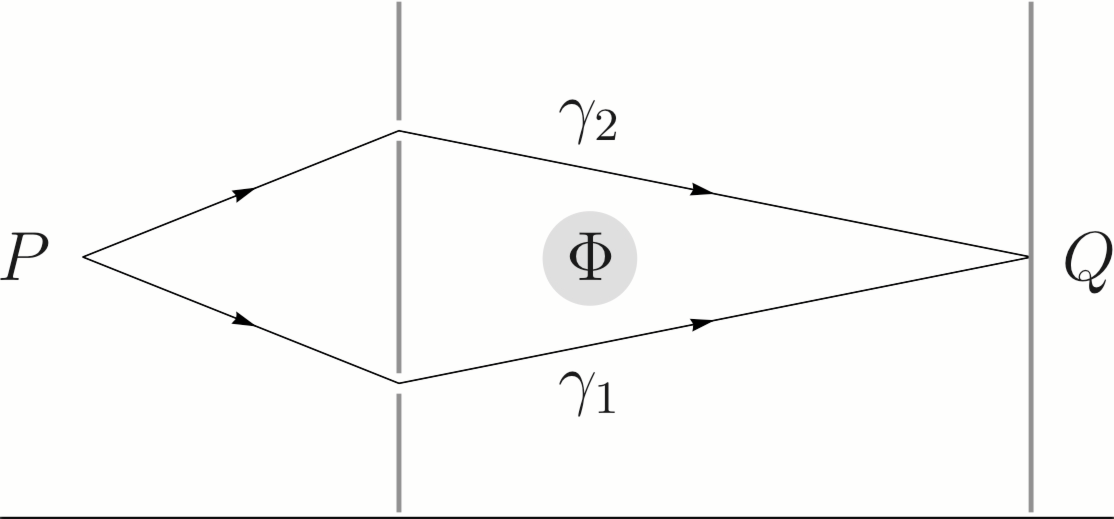
\includegraphics[width=9cm, height=5cm]{AB.png}
    \caption{Aharonov-Bohm double slit experiment}
    \label{fig:1}
\end{figure}

Then let's get down to the main experiment. Let's see the figure~\ref{fig:1}.
Figure~\ref{fig:1} is simple diagram of Aharonov-Bohm experiment. The description of experiment is: \cite{experiment}
\begin{quote}
\textit{Consider the above plan view of the classic double-slit experiment, consisting of a source P of identical particles
each having a charge q (electrons will do nicely), an impenetrable screen with two closely-spaced, narrow slits,
and a detector Q. In practice, the slit widths will be on the order of several microns, separated by a section of
screen of comparable dimension. Such small distances are necessary in view of the quantum nature of the double
slit experiment itself. In addition, we place a solenoid ($\it\Phi$) immediately behind the slit separation. The solenoid
itself must be extremely small, and the ends must be shielded in such a way as to prevent any ‘‘fringe’’ interaction
with the charged particles.}
\end{quote}
Since the solenoid is completely shielded, there is no magnetic field in outside of solenoid, so there shouldn't be any "fringe" interaction in classical mechanics. But in quantum world, it's trivial to exist a fringe interaction. Before dealing with AB effect, let consider path integral for two path free particle. By \eqref{eq:5}, transition amplitudes for each path is given as:
\begin{equation}\label{eq:7}
\begin{split}
&U_1=A\int_{\gamma_1}\mathcal{D}x\ e^{\frac{i\mathcal{S}_0}{\hbar}}\\
&U_2=A\int_{\gamma_2}\mathcal{D}x\ e^{\frac{i\mathcal{S}_0}{\hbar}}
\end{split}
\end{equation}
Since, these paths are free particle's so, we can separate $U$ as amplitude term and phase term.
\begin{equation}\label{eq:8}
\begin{split}
&U_1=\Big(\frac{m}{2\pi i\hbar t}\Big)^{\frac{1}{2}}\exp\Big(\frac{i\theta_1}{\hbar}\Big)\\
&U_2=\Big(\frac{m}{2\pi i\hbar t}\Big)^{\frac{1}{2}}\exp\Big(\frac{i\theta_2}{\hbar}\Big)
\end{split}
\end{equation}
Thus the total transition amplitude \(U=U_1+U_2\) is obtained: 
\begin{equation}\label{eq:9}
U=\Big(\frac{m}{2\pi i\hbar t}\Big)^{\frac{1}{2}}\exp\Big(\frac{i\theta_1}{\hbar}\Big)[1+\exp(i\Delta)]
\end{equation}
$\Delta$ means phase difference of two paths (\(\Delta=\frac{\theta_2-\theta_1}{\hbar}\)). Now, we are interested in transition probability, so, let use the relation $P\propto |U|^2$. Then only a little bit calculation is needed to show that:
\begin{equation}\label{eq:10}
|U|^2=\frac{2m}{\pi\hbar t}\cos^2\Big(\frac{1}{2}\Delta\Big)
\end{equation}

In this time, we calculate transition amplitude which includes EM interaction. By \eqref{eq:6}, transition amplitude is given as:
\begin{equation}\label{eq:11}
U_n=\Big(\frac{m}{2\pi i\hbar t}\Big)^{\frac{1}{2}}\exp\Big(\frac{i\theta_n}{\hbar}\Big)\exp\Big(\frac{iq}{\hbar c}\int_{\gamma_n}A_i\ dx^i\Big)
\end{equation}
Using \(U=U_1+U_2\) then:
\begin{multline}\label{eq:12}
U=\Big(\frac{m}{2\pi i\hbar t}\Big)^{\frac{1}{2}}\exp\Big(\frac{i\theta_1}{\hbar}\Big)\exp\Big(\frac{iq}{\hbar c}\int_{\gamma_1}A_i\ dx^i\Big)\\ \Big[1+\exp(i\Delta)\exp\Big[\frac{iq}{\hbar c} \Big(\int_{2}A_i\ dx^i - \int_{1}A_i\ dx^i \Big)\Big]\Big]
\end{multline}
By \(\int_{1}A_i\ dx^i - \int_{2}A_i\ dx^i=\oint A_i\ dx^i=\iint \vec{B}\cdot\hat{n}dS=\Phi_B\), the transition amplitude is:
\begin{multline}\label{eq:13}
U=\Big(\frac{m}{2\pi i\hbar t}\Big)^{\frac{1}{2}}\exp\Big(\frac{i\theta_1}{\hbar}\Big) \exp\Big(\frac{iq}{\hbar c}\int_{\gamma_1}A_i\ dx^i\Big)\\ \Big[1+\exp(i\Delta)\exp\Big(-\frac{iq}{\hbar c} \Phi_B\Big)\Big]
\end{multline}
Finally, calculate $|U|^2$ then we can get following relation.
\begin{equation}\label{eq:14}
|U|^2=\frac{2m}{\pi\hbar t}\cos^2\Big[\frac{1}{2}\Big(\Delta-\frac{q\Phi_B}{\hbar c}\Big)\Big]
\end{equation}
\begin{equation}\label{eq:15}
\therefore\Delta\ \rightarrow\ \Delta-\frac{q\Phi_B}{\hbar c}
\end{equation}

Eq.\eqref{eq:15} is just Aharonov-Bohm effect. Although there is no magnetic field, the phase shift can be observed. It means, the vector potential affects to real space. Therefore the vector potential is physically real variable.

\section{\label{sec:level3}Berry Phase}
\subsection{\label{sec:level3.1}Parallel transport}
To understand berry phase starts from understanding parallel transport. In fact, a concept of parallel transport is very simple. First, let take a basis vector which tangent to curve $\mathcal{C}$. It means, let $\hat{n}$ be a normal vector of plane which includes curve $\mathcal{C}$. Then \(\hat{n}\cdot e^r=0\). And It should hold norm, so, \(\dot{e}^r=\omega\times e^r \rightarrow e^r \cdot \dot{e}^r=0\). Let define second basis by \(e^2 = n \times e^1\) and define new basis vector by combine two bases:
\[\Phi=\frac{e^1 + ie^2}{\sqrt{2}}\]
Then we can get the following relation.\cite{pt}
\begin{equation}\label{eq:16}
\phi^{*}\dot{\phi}=0
\end{equation}
Eq.\eqref{eq:16} represents parallel transport.

The geometric phase $\theta(\mathcal{C})$ occurs at transforming this result - moving frame to fixed frame (\(\phi(t)=e^{-i\theta(t)}u(r)\)). And let substitute this to eq.\eqref{eq:16}, then we can get what $\theta$ is.
\begin{equation}\label{eq:17}
\begin{split}
&\dot{\theta}=\Im(u^*\dot{u})\\
&\theta(\mathcal{C})=\Im\oint_{\mathcal{C}}u^*\cdot du
\end{split}
\end{equation}
Let define new vector field $A_i(x)$.
\[A_i(x)=\Im[\tensor{u}{_j^*}(x)\partial_i u_j(x)]\]
Then we can rewrite the geometric phase $\theta(\mathcal{C})$ as:
\begin{equation}\label{eq:18}
\theta(\mathcal{C})=\Im\oint_{\mathcal{C}}A_i(x)\cdot d\vec{x}
\end{equation}
Add some calculation, we can see that $\theta(\mathcal{C})$ corresponds to solid angle (see \cite{pt}). Thus, it's reasonable to name $\theta(\mathcal{C})$ to the geometric phase.\\

\subsection{\label{sec:level3.2}Parallel transport in Quantum mechanics}

Consider the adiabatic quantum system. Then, we can write the state as:
\begin{equation}\label{eq:19}
\ket{\psi(t)}=\exp\Big(-\frac{i}{\hbar}\int_{0}^{t} E_n(r(t'))\ dt'\Big)\ket{\phi(t)}
\end{equation}
Let substitute eq.\eqref{eq:19} to schr{\"o}dinger equation and apply adiabatic theorem (\(H\ket{\psi(t)}=E_n\ket{\psi(t)}\)). Then we can get next relation:
\begin{equation}\label{eq:20}
\braket{\phi_n(t)|\dot{\phi}_n(t)}=0
\end{equation}
Let compare this to eq.\eqref{eq:16} then it is trivial that eq.\eqref{eq:20} represents parallel transport in QM. Then, also, we transform moving frame to fixed frame:
\begin{equation}\label{eq:21}
\ket{\phi_n(t)}\equiv\exp(i\gamma_n(t))\ket{n(R)}
\end{equation}
$\gamma_n(\mathcal{C})$ is called \textit{Berry Phase.} By the relation \eqref{eq:17}, Berry phase has the form: ($\gamma\simeq-\theta$)
\begin{equation}\label{eq:22}
\gamma_n(\mathcal{C})=-\Im\Big[\oint_{\mathcal{C}}\bra{n(R)}\partial_R\ket{n(R)}\cdot dR \Big]
\end{equation}
Also, let define new variable $A^n(R)$.
\[A^n(R)\equiv-\Im\braket{n(R)|\partial_R n(R)}\]
Then let substitute this to eq.\eqref{eq:22} then we can get the berry phase.
\begin{equation}\label{eq:23}
\gamma_n(\mathcal{C})=\oint_{\mathcal{C}}A^n(R)\ \cdot dR
\end{equation}

\subsection{\label{sec:level3.3}Connection between Aharonov-Bohm effect and Berry phase}

\begin{figure}[h]
    \centering
    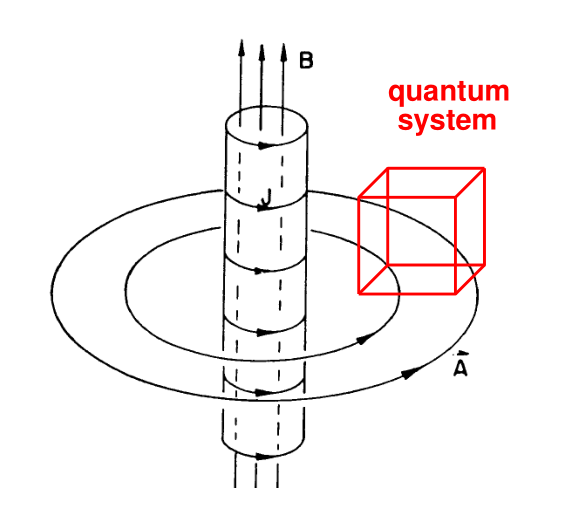
\includegraphics[width=9cm, height=5cm]{AB2.png}
    \caption{Aharonov-Bohm effect given by Berry\cite{RR}}
    \label{fig:2}
\end{figure}

Now, let's combine concepts of AB effect and Berry phase. To do this, we need to imagine quantum system like fig~\ref{fig:2}. Let $R$ be a distance from origin to box and r be a main distance from origin to particle. Then the Hamiltonian describing the particles in the box is \(H(p,r-R)\) with corresponding wave function $\psi_n(r-R)$ \cite{pt}. When the flux is non-zero, then we can take a basis states $\ket{n(R)}$, such that
\begin{equation}\label{eq:24}
H(p-qA(r),\ r-R)\ket{n(R)}=E_n\ket{n(R)} 
\end{equation}
The solution of eq.\eqref{eq:24} is given by
\begin{equation}\label{eq:25}
\braket{r|n(R)}=\exp\Big[\frac{iq}{\hbar c}\int_{R}^{r} A(r')\cdot dr'\Big]\psi_n(r-R)
\end{equation}
Then let calculate Berry phase using the relation \eqref{eq:23}. To calculate, we need to obtain $A^n(R)$ first. By the definition of $A^n(R)$,
\begin{multline}\label{eq:26}
\begin{split}
A^n(R)&= -\Im[\braket{n(R)|\partial_Rn(R)}]\\
&= -\Im\Big[\iiint d^3r\ \tensor{\psi}{_n^*}(r-R)\\
&\quad \Big[\frac{-iq}{\hbar c}A(R)\psi_n(r-R)+\partial_R\psi_n(r-R)\Big]\Big]
\\ &= \frac{q}{\hbar c}A(R)
\end{split}
\end{multline}
Thus, Berry phase can be obtained as
\begin{equation}\label{eq:27}
\gamma_n(\mathcal{C})=\frac{q}{\hbar c}\oint_{\mathcal{C}}A(R)\cdot dR
\end{equation}
And it is same as eq.\eqref{eq:12} - path integral prediction. 
And so on, it is same that $\frac{q}{\hbar c}\Phi_B$.
Therefore, phase shift of Aharonov-Bohm effect can be rewritten as
\begin{equation}\label{eq:28}
\therefore \Delta\ \rightarrow\ \Delta-\gamma(\mathcal{C})
\end{equation}

\section{\label{sec:level4}Discussion}

\subsection{\label{sec:level4.1}Methodology}

We did the path integral approach to Aharonov-Bohm effect and connection between AB effect and the berry phase. And the result says two alternative methods converge to same conclusion. It's important to understand two major methods of Quantum mechanics - path integral, canonical formalism. And Aharonov-Bohm effect is good example to do this. Path integral gives us physical meanings by more intuitive ways and canonical formalism (Here, it means normal strategy) gives us relations between operators and states. Then we can quantize physics easier.

\subsection{\label{sec:level4.2}Aharonov-Bohm effect}

During study physics, we should be surrounded by plenty of symmetries and transforms. And sometimes we may ask ourselves - What is the meaning of these?
Scalar and vector potential in Electromagnetism are good example of this problem. We use gauge transform (maybe $U(1)$ global transform) infinitely many, but we can't usually answer to what's physical meaning of scalar or vector potential? 
Aharonov-Bohm effect is awesome solution of these questions. The vector potential is not only abstract vector field but also physical observable. So, any gauge choice is not more fundamental than others. And also it can be evidence that fields also can be observables. So, it expands our understanding from QM to QFT smoothly.

\begin{thebibliography}{9}
\bibitem{Berry}
M.V. Berry. \textit{Quantal Phase Factors Accompanying Adiabatic Changes} Proc. Roy. Soc. London A 392, 45 (1984).

\bibitem{Pancharatnam}
S. Pancharatnam, Proceedings of the Indian Academy in Sciences, 44, 247 (1956).

\bibitem{Foucault}
J.H. Hannay, J. Phys. A: Math. Gen. 18, 221 (1985).

\bibitem{Aharonov}
Y. Aharonov, D. Bohm. \textit{Significance of electromagnetic potentials in the quantum theory.} Phys. Rev. 115(3):485, (1959).

\bibitem{experiment}
Tonomura, A. et al. \textit{Evidence for Aharonov-Bohm effect with magnetic field completely shielded from electron wave.} Phys. Rev. 56: 792$-$795 (1986).

\bibitem{pt}
P. Bruno, \textit{Berry phase effects in magnetism}, “Magnetism goes nano”, 36th Spring School of the Institute of Solid State Research (Jülich), edited by Stefan Blügel, Thomas Brückel, and Claus M. Schneider, pp. E9.1 – E9.33, Forschungszentrum Jülich (2005)

\bibitem{RR}
 R. Resta, \textit{Manifestations of Berry’s phase in molecules and in condensed matter}, J. Phys.: Condens. Matter 12, R107 (2000).

\end{thebibliography}
\end{document}
%
% ****** End of file apssamp.tex ******
